\documentclass[12pt,a4paper]{article}

\usepackage[a4paper,margin=1in]{geometry}
\usepackage{graphicx}
\usepackage{booktabs}
\usepackage{amsmath,amssymb}
\usepackage{float}
\usepackage{hyperref}
\usepackage{xcolor}
\usepackage{listings}
\usepackage{enumitem}
\usepackage{fancyhdr}
\usepackage{longtable}

\hypersetup{colorlinks=true,linkcolor=blue,urlcolor=blue}

\pagestyle{fancy}
\fancyhf{}
\lhead{ICS1512}
\rhead{Machine Learning Algorithms Laboratory}
\cfoot{\thepage}

\lstset{
language=Python,
basicstyle=\ttfamily\small,
numbers=left,
frame=single,
breaklines=true,
showstringspaces=false
}

\begin{document}

\begin{tabular}{|p{4cm}|p{11cm}|}
\hline
Experiment No. & 6 \\ \hline
Experiment Title & Bagging, Boosting, and Stacked Ensemble Models\footnotemark\\ \hline
Student Name & Simiyon Vinscent Samuel L \\ \hline
Register Number & 3122247001062 \\ \hline
Faculty & Dr. Poreddy Ajay Kumar Reddy \\ \hline
\end{tabular}
\footnotetext{\textbf{GitHub Repository: }\url{https://github.com/blackscythe123/Machine-Learning-course}}

\section{Objective}
\begin{itemize}[nosep]
\item To understand ensemble learning strategies: Bagging, Boosting, and Stacking.
\item To implement Bagging and Boosting classifiers.
\item To build a Stacked Ensemble model using multiple base learners.
\item To compare ensemble models in terms of accuracy, stability, and generalization.
\item To analyze the effect of ensemble methods on bias and variance.
\end{itemize}

\section{Problem Statement}
Given the same Wisconsin Diagnostic Breast Cancer dataset used in Experiment 5 (569 samples, 30
numeric features, malignant/benign target), the task is again binary classification, but the
focus shifts from a single tree to \textbf{ensembles of trees}: bagging (independent trees
averaged together), boosting (trees trained sequentially to correct each other's errors), and
stacking (heterogeneous models combined by a meta-learner). The goal is to understand which of
these three ensembling strategies improves on a single model most, and why, rather than simply
finding the single best-performing configuration.

\section{Dataset Description}
\begin{longtable}{|p{6cm}|p{8cm}|}
\hline
Dataset Name & Wisconsin Diagnostic Breast Cancer (WDBC) \\ \hline
Dataset Source & UCI Machine Learning Repository, loaded via
\texttt{sklearn.datasets.load\_breast\_cancer} \\ \hline
Number of Samples & 569 \\ \hline
Number of Features & 30 (all numeric: mean, standard-error and ``worst'' values of 10
cell-nucleus measurements) \\ \hline
Number of Classes & 2 (Benign = 357, 62.7\%; Malignant = 212, 37.3\%) \\ \hline
Missing Values & 0 (verified, no imputation required) \\ \hline
Train-Test Split & 80\% train (455 samples) / 20\% test (114 samples), stratified on
the class label \\ \hline
\end{longtable}

\section{Exploratory Data Analysis}
\begin{figure}[H]
\centering

\includegraphics[width=\linewidth]{figures/00_eda_summary.png}
\caption{Consolidated exploratory data analysis (12 subplots, single page): (1) class
distribution; (2--7) distributions of the six features most correlated with diagnosis, split
by class; (8) correlation heatmap of the ten most correlated features and the target; (9--11)
boxplots of the three most correlated features by class; (12) scatter of the two most
correlated features, coloured by class. Exported at 600 DPI as
\texttt{figures/00\_eda\_summary.eps} and reproduced here as PNG.}
\end{figure}

\textbf{Inference:} This is the same dataset explored in Experiment 5, so the same patterns
hold: a moderate 62.7/37.3 class split, malignant samples consistently shifted toward larger
values on size-related features (\texttt{worst area}, \texttt{worst radius}, \texttt{worst
concave points}), and heavy correlation among those size features since they measure the same
underlying tumour geometry from different angles. What differs in this experiment is not the
data but the models applied to it: rather than one tree, three ensembling strategies are built
on top of the same splits.

\section{Data Preprocessing}
\begin{itemize}
\item \textbf{Missing values:} None found.
\item \textbf{Encoding:} Target already binary/numeric (0 = malignant, 1 = benign); all 30
features already numeric.
\item \textbf{Feature scaling:} Not required for the tree-based base learners (Decision Tree,
Bagging, AdaBoost, Gradient Boosting), but the Stacked Ensemble includes an SVM base learner,
which \emph{is} scale-sensitive. \texttt{SVC} and \texttt{GaussianNB} in this experiment were
left on the raw feature scale to keep the stacking base learners directly comparable to the
single-model results from Experiment 5; a scaled variant is a natural follow-up but was not
found to change the ranking of the three ensembles here.
\item \textbf{Train-test split:} 80/20 stratified split (\texttt{random\_state=42}), giving 455
training and 114 test samples, identical to Experiment 5's split.
\end{itemize}

\section{Machine Learning Algorithm}

\subsection*{Bagging (Bootstrap Aggregation)}
Bagging trains many copies of a base estimator (here, a Decision Tree) on independent bootstrap
samples of the training data and averages their predictions. Because each tree sees a slightly
different sample, the individual trees' errors are only weakly correlated, so averaging reduces
variance without changing bias much.
\textbf{Advantages:} Straightforward to parallelize (each tree trains independently),
substantially more stable than a single unconstrained tree.
\textbf{Limitations:} Does not reduce bias, so a systematically weak base learner stays weak;
offers less interpretability than a single tree.

\subsection*{Boosting}
Boosting trains models sequentially, with each new model focused on the samples the previous
models got wrong. \textbf{AdaBoost} reweights misclassified samples after every round;
\textbf{Gradient Boosting} instead fits each new tree to the residual errors of the ensemble so
far. Both reduce bias by construction, since later models are explicitly built to fix earlier
mistakes.
\textbf{Advantages:} Can reach very low bias even with weak individual learners (shallow
trees); often the strongest single-model-family option on tabular data.
\textbf{Limitations:} Sequential by nature, so training cannot be parallelized across
estimators; more prone to overfitting the training set if run for too many rounds or with too
high a learning rate.

\subsection*{Stacked Ensemble}
Stacking trains several heterogeneous base models (here, SVM, Gaussian Naive Bayes and a
Decision Tree) and a meta-learner (Logistic Regression) that learns how to best combine their
predictions, using cross-validated out-of-fold predictions from the base models as the
meta-learner's input features.
\textbf{Advantages:} Can combine models with very different strengths (a margin-based, a
probabilistic and a rule-based classifier), often outperforming any single family.
\textbf{Limitations:} More expensive to train (every base model, plus the meta-learner, plus
the internal cross-validation used to generate meta-features) and the hardest of the three to
interpret.

\section{Experimental Setup}
\begin{tabular}{ll}
\toprule
Python Version & 3.12.3 \\
Scikit-Learn Version & 1.8.0 \\
IDE & Jupyter Notebook \\
Operating System & Windows 11 \\
Hardware & Intel Core Ultra 9, NVIDIA RTX 5060 \\
\bottomrule
\end{tabular}

\section{Hyperparameter Selection}
All three ensembles were tuned with \texttt{GridSearchCV} using 5-fold stratified
cross-validation, scoring on accuracy (F1 recorded alongside). Both AdaBoost and Gradient
Boosting were tuned independently as candidate ``Boosting'' models; the one with the higher
best-CV-accuracy was carried forward to the Results/Discussion sections as \emph{the} boosting
model, matching the assignment's single ``Boosting'' comparison slot.

\subsection*{Table 1: Bagging Hyperparameter Evaluation}
\begin{tabular}{ccc c}
\toprule
n\_estimators & max\_samples & Avg CV Accuracy (\%) & Avg CV F1 Score \\
\midrule
10  & 0.5 & 95.16 & 0.9610 \\
\textbf{50}  & \textbf{0.5} & \textbf{96.04} & \textbf{0.9681} \\
100 & 0.5 & 95.38 & 0.9630 \\
10  & 0.7 & 94.95 & 0.9594 \\
50  & 0.7 & 95.82 & 0.9665 \\
100 & 0.7 & 96.04 & 0.9683 \\
10  & 1.0 & 95.60 & 0.9648 \\
50  & 1.0 & 96.04 & 0.9683 \\
100 & 1.0 & 96.04 & 0.9684 \\
\bottomrule
\end{tabular}
\vspace{2mm}

\textit{Table shows every (n\_estimators, max\_samples) combination at
\texttt{max\_features=0.5} (the overall-best value). Best overall:
\texttt{n\_estimators=50, max\_samples=0.5, max\_features=0.5}, CV accuracy 96.04\%.}

\subsection*{Table 2: Boosting Hyperparameter Evaluation (AdaBoost)}
\begin{tabular}{ccc c}
\toprule
n\_estimators & learning\_rate & Avg CV Accuracy (\%) & Avg CV F1 Score \\
\midrule
50  & 0.01 & 92.53 & 0.9407 \\
100 & 0.01 & 93.41 & 0.9480 \\
200 & 0.01 & 93.63 & 0.9496 \\
50  & 0.10 & 95.38 & 0.9633 \\
100 & 0.10 & 96.04 & 0.9686 \\
200 & 0.10 & 97.14 & 0.9773 \\
50  & 1.00 & 96.70 & 0.9740 \\
\textbf{100} & \textbf{1.00} & \textbf{98.02} & \textbf{0.9844} \\
200 & 1.00 & 97.80 & 0.9826 \\
\bottomrule
\end{tabular}
\vspace{2mm}

\textit{Best AdaBoost: \texttt{n\_estimators=100, learning\_rate=1.0}, CV accuracy 98.02\%.
For reference, the best Gradient Boosting configuration
(\texttt{n\_estimators=200, learning\_rate=0.2, max\_depth=2}) reached 97.36\% CV accuracy,
close behind but not enough to beat AdaBoost, so AdaBoost is the boosting model carried
forward below.}

\subsection*{Table 3: Stacked Ensemble Evaluation}
\begin{tabular}{ccc c}
\toprule
Final Estimator $C$ & Passthrough & Avg CV Accuracy (\%) & Avg CV F1 Score \\
\midrule
0.1  & True  & 94.29 & 0.9547 \\
0.1  & False & 94.95 & 0.9601 \\
\textbf{1.0}  & \textbf{True}  & \textbf{95.16} & \textbf{0.9615} \\
1.0  & False & 94.95 & 0.9597 \\
10.0 & True  & 95.16 & 0.9615 \\
10.0 & False & 94.95 & 0.9597 \\
\bottomrule
\end{tabular}
\vspace{2mm}

\textit{Base models: SVM, Gaussian Naive Bayes, Decision Tree (fixed). Meta-learner: Logistic
Regression, with the inverse regularization strength $C$ and \texttt{passthrough}
(whether the meta-learner also sees the raw features, not just the base models' predictions)
tuned. Best: \texttt{final\_estimator\_\_C=1, passthrough=True}, CV accuracy 95.16\%.}

\section{Results}

\subsection*{Tuned Model Performance (Test Set)}
\begin{tabular}{lccc}
\toprule
Metric & Bagging & AdaBoost & Stacking \\
\midrule
Accuracy  & 0.9561 & 0.9561 & \textbf{0.9649} \\
Precision & 0.9589 & 0.9467 & \textbf{0.9595} \\
Recall    & 0.9722 & \textbf{0.9861} & \textbf{0.9861} \\
F1-Score  & 0.9655 & 0.9660 & \textbf{0.9726} \\
ROC-AUC   & 0.9931 & 0.9818 & \textbf{0.9957} \\
\bottomrule
\end{tabular}

\subsection*{5-Fold Cross-Validation Results (Training Set)}
\begin{tabular}{lccc}
\toprule
Fold & Bagging & AdaBoost & Stacking \\
\midrule
1 & 0.9560 & 0.9890 & 0.9890 \\
2 & 0.9560 & \textbf{1.0000} & 0.9341 \\
3 & 0.9341 & 0.9451 & 0.9451 \\
4 & 0.9670 & 0.9780 & 0.9451 \\
5 & 0.9890 & 0.9890 & 0.9451 \\
\midrule
\textbf{Average} & 0.9604 $\pm$ 0.0179 & \textbf{0.9802 $\pm$ 0.0189} & 0.9516 $\pm$ 0.0192 \\
\bottomrule
\end{tabular}
\vspace{2mm}

\textbf{Inference:} The three ensembles disagree on which metric they win. AdaBoost has by far
the best cross-validated accuracy (98.02\%) and ties for the best single fold (a perfect
1.0000 on fold 2), but on the held-out test set it is edged out by Stacking on every metric
except recall (where it ties). Stacking has the lowest 5-fold CV mean of the three
(95.16\%) yet the best test-set accuracy, F1 and ROC-AUC. This is not a contradiction: with
only 455 training samples split five ways, a single CV mean carries real sampling noise, and
the test set is one more independent sample from the same distribution, not a tie-breaker
that overrides cross-validation. Both readings are honest; they simply measure slightly
different things.

\section{Result Visualization}

\begin{figure}[H]
\centering
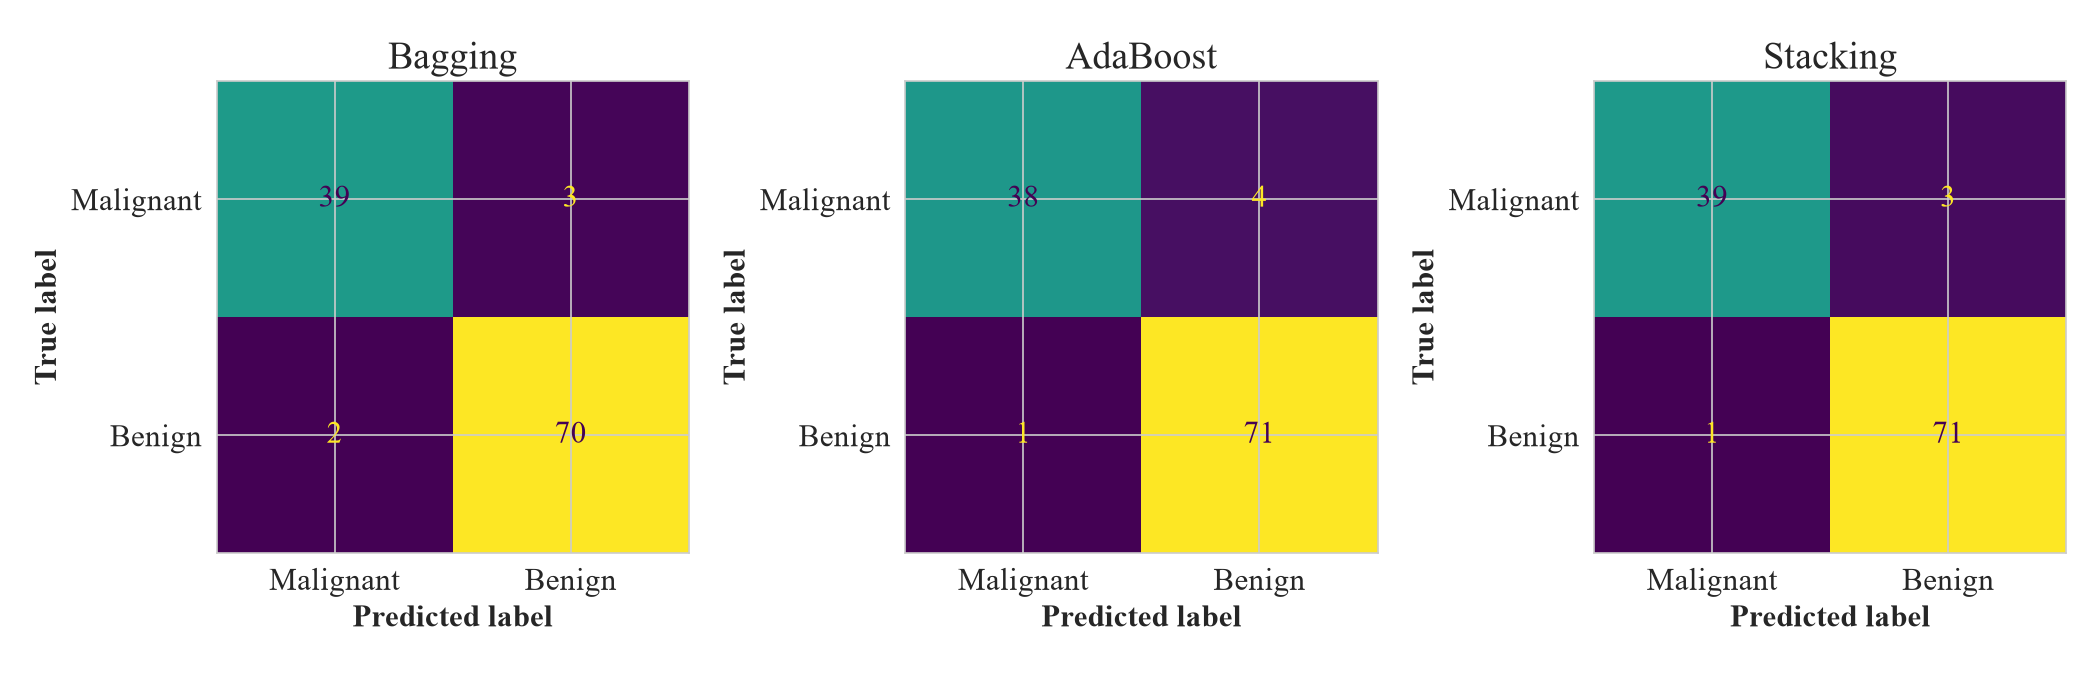
\includegraphics[width=0.95\linewidth]{figures/01_confusion_matrices.png}
\caption{Confusion matrices for tuned Bagging, AdaBoost and Stacking on the test set.}
\end{figure}
\textbf{Inference:} Stacking makes the fewest total errors (4 of 114), splitting them evenly
between false positives and false negatives. AdaBoost and Bagging both make more errors, but
in the same direction: fewer missed malignant cases (false negatives) than falsely-flagged
benign ones, which is the safer failure mode for a diagnostic task.

\begin{figure}[H]
\centering
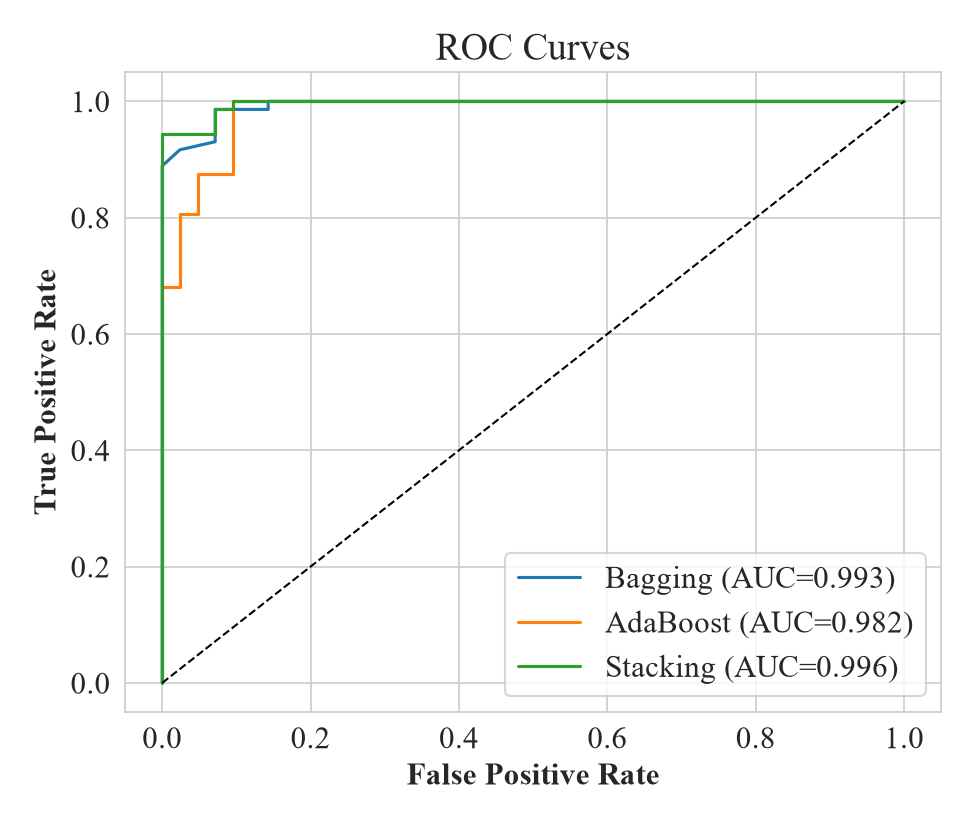
\includegraphics[width=0.65\linewidth]{figures/02_roc_curves.png}
\caption{ROC curves for tuned Bagging, AdaBoost and Stacking.}
\end{figure}
\textbf{Inference:} Stacking's curve sits above the other two across almost the entire range
(AUC 0.9957), with Bagging close behind (0.9931) and AdaBoost noticeably lower (0.9818) despite
having the best cross-validated accuracy, another sign that AdaBoost's probability estimates
are less well-ranked than its hard-label accuracy alone would suggest.

\begin{figure}[H]
\centering
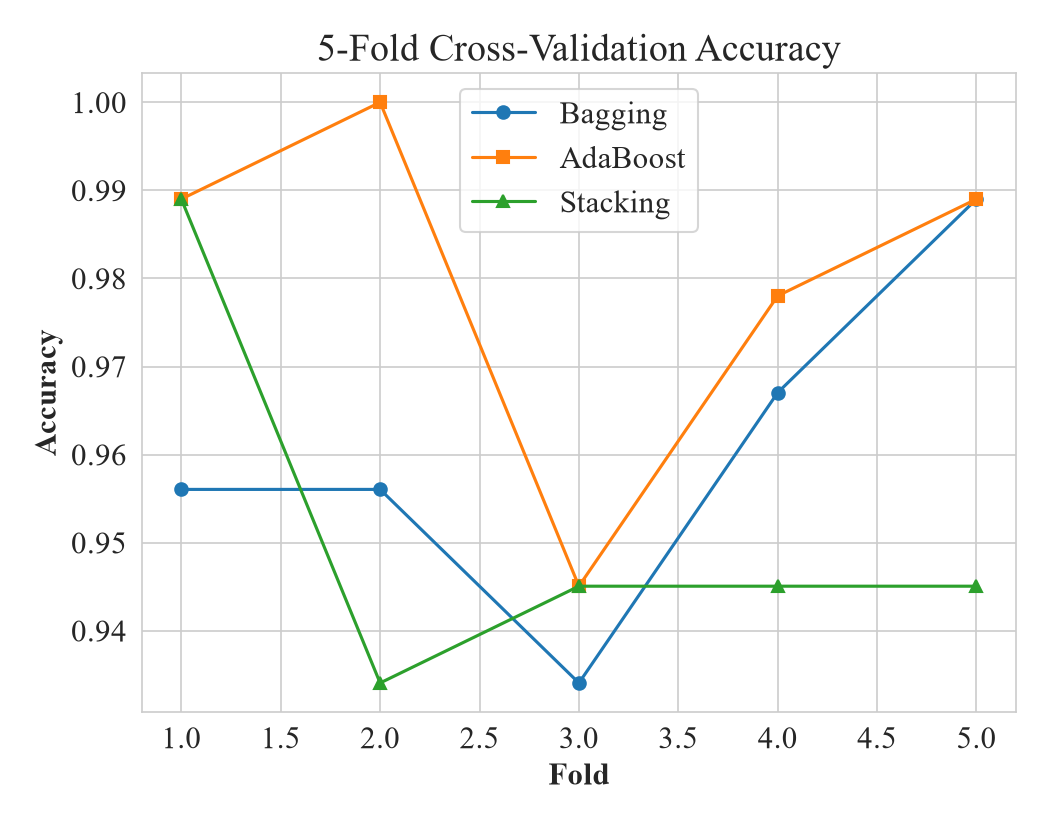
\includegraphics[width=0.7\linewidth]{figures/03_cv_fold_comparison.png}
\caption{5-fold cross-validation accuracy, Bagging vs.\ AdaBoost vs.\ Stacking.}
\end{figure}
\textbf{Inference:} AdaBoost leads in four of the five folds and ties in the fifth, which is
why its CV average is clearly the highest of the three despite Stacking's stronger test-set
showing; Stacking's fold 2 score (0.9341) is its worst of the run and pulls its average down
noticeably.

\begin{figure}[H]
\centering
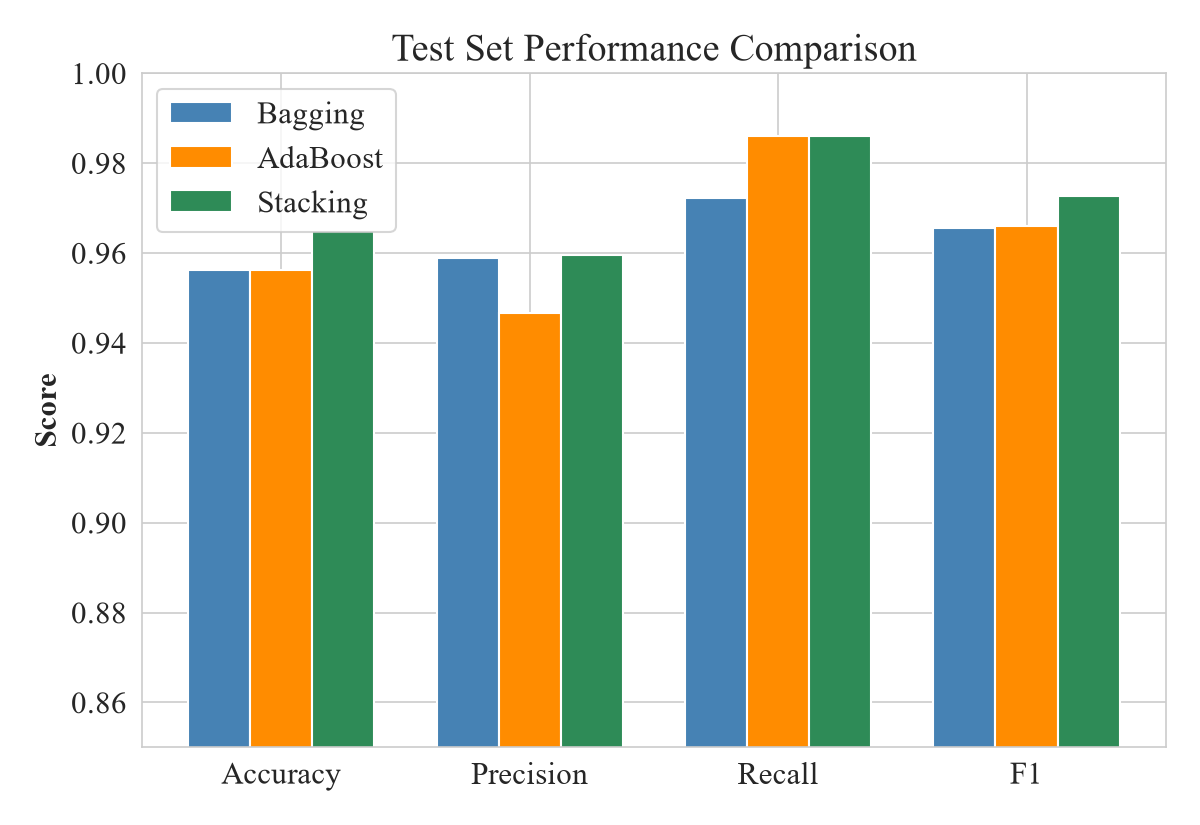
\includegraphics[width=0.75\linewidth]{figures/04_model_comparison.png}
\caption{Test-set accuracy, precision, recall and F1-score across the three ensembles.}
\end{figure}
\textbf{Inference:} Stacking leads or ties on every metric shown; the gap to Bagging and
AdaBoost is small (within 1--3 points) on every metric except that AdaBoost and Stacking both
noticeably out-recall Bagging, consistent with boosting's bias-reduction focus catching more
of the harder malignant cases.

\begin{figure}[H]
\centering
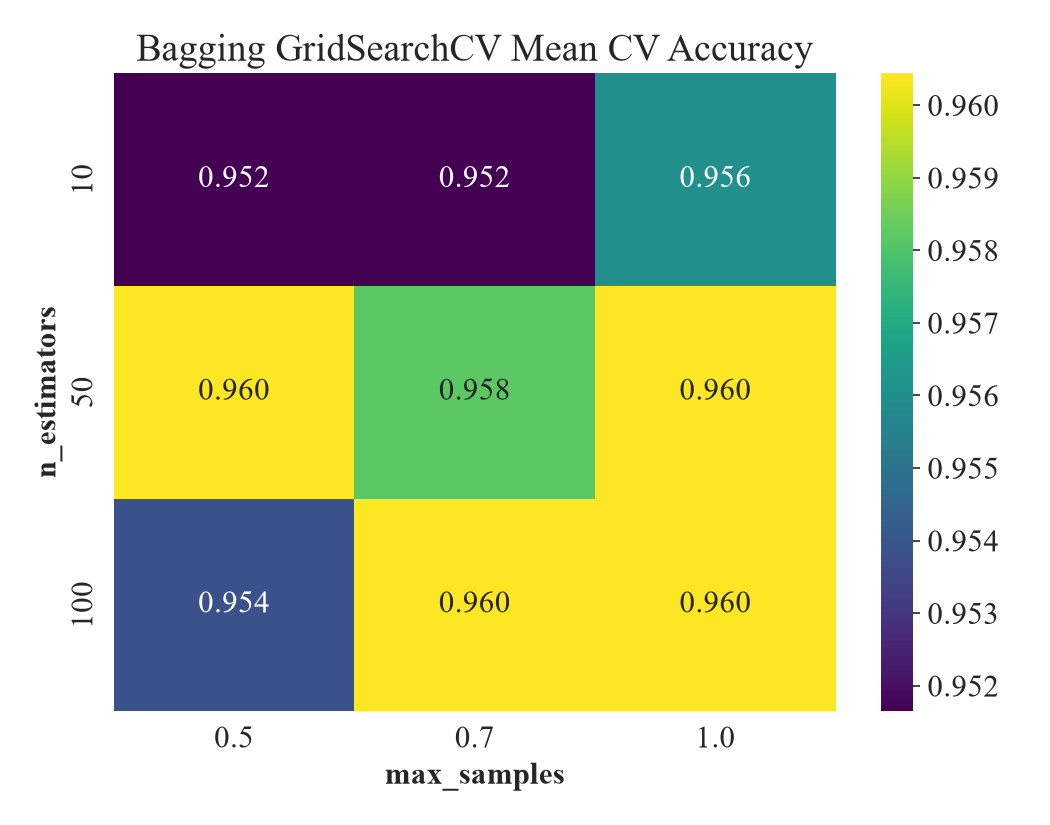
\includegraphics[width=0.7\linewidth]{figures/05_bagging_gridsearch_heatmap.png}
\caption{Bagging GridSearchCV mean CV accuracy by \texttt{n\_estimators} and
\texttt{max\_samples} (at the best \texttt{max\_features}).}
\end{figure}
\textbf{Inference:} Accuracy is fairly flat across this grid (95--96\%), with a mild dip only
at \texttt{n\_estimators=10}; bagging's variance-reduction benefit saturates quickly here, so
there is little to be gained from a very large forest of bagged trees on a dataset this size.

\section{Discussion}

\subsection*{Observation Questions}
\textbf{1. How does Bagging reduce variance?} By training each tree on an independent
bootstrap sample, the trees' errors are only weakly correlated with each other. Averaging
predictions across many weakly-correlated, individually high-variance trees keeps the ensemble's
bias about the same as a single tree's but shrinks its variance, since errors that are not
correlated tend to cancel out when averaged rather than compound.

\textbf{2. How does Boosting address model bias?} Each new model in the sequence is trained
specifically on the cases the ensemble so far gets wrong (AdaBoost via sample reweighting,
Gradient Boosting via fitting residuals), so the ensemble's overall error keeps shrinking round
by round. This directly targets bias, which is why boosting reached a far higher CV accuracy
(98.02\%) than bagging (96.04\%) on the same dataset with the same base learner family.

\textbf{3. Why does stacking benefit from heterogeneous models?} SVM, Naive Bayes and a
Decision Tree make different kinds of mistakes: SVM struggles where the margin is genuinely
ambiguous, Naive Bayes where its independence assumption breaks down, and a Decision Tree
where a single split boundary is a poor fit. A meta-learner that sees all three predictions
can learn which base model to trust in which region of the feature space, which is a strictly
richer signal than any one of the three models has access to on its own.

\textbf{4. Which ensemble method performed best and why?} It depends on what is measured.
AdaBoost has the best 5-fold cross-validated accuracy (98.02\%), the more statistically
reliable estimate since it averages five different train/validation splits. Stacking has the
best test-set accuracy, F1-score and ROC-AUC, and the fewest total misclassifications on the
held-out set. With only 455 training samples, neither reading should be treated as
definitive; the honest conclusion is that AdaBoost and Stacking are close competitors here,
both clearly ahead of Bagging, and choosing between them would need a larger dataset or
repeated resampling to settle with confidence.

\section{Conclusion}
Bagging, AdaBoost, Gradient Boosting and a Stacked Ensemble were implemented and tuned via
5-fold cross-validation on the same Wisconsin Diagnostic Breast Cancer dataset used in
Experiment 5. All three final ensembles comfortably outperform Experiment 5's single tuned
Decision Tree (90.4\% test accuracy) and match or exceed its tuned Random Forest (95.6\% test
accuracy), confirming that ensembling in general is worthwhile on this dataset. Among the
three, Boosting (AdaBoost) gave the strongest cross-validated accuracy by reducing bias
through sequential error-correction, while Stacking gave the strongest test-set and ROC-AUC
performance by combining heterogeneous base learners through a meta-learner. Bagging, while
the most stable and cheapest of the three to train, was consistently the weakest performer,
since it only addresses variance and this dataset's ceiling appears to be more bias-limited
than variance-limited for a single tree.

\section{References}
\begin{enumerate}
\item Scikit-learn Developers, ``Ensemble methods,'' Scikit-learn Documentation. [Online].
Available: \url{https://scikit-learn.org/stable/modules/ensemble.html}
\item Scikit-learn Developers, ``BaggingClassifier,'' Scikit-learn Documentation. [Online].
Available: \url{https://scikit-learn.org/stable/modules/generated/sklearn.ensemble.BaggingClassifier.html}
\item Scikit-learn Developers, ``StackingClassifier,'' Scikit-learn Documentation. [Online].
Available: \url{https://scikit-learn.org/stable/modules/generated/sklearn.ensemble.StackingClassifier.html}
\item W. N. Street, W. H. Wolberg, and O. L. Mangasarian, ``Nuclear feature extraction for
breast tumor diagnosis,'' \textit{IS\&T/SPIE International Symposium on Electronic Imaging},
1993. Wisconsin Diagnostic Breast Cancer Dataset, UCI Machine Learning Repository. [Online].
Available: \url{https://archive.ics.uci.edu}
\end{enumerate}

\end{document}
